\section{ニューラルネットワークの学習}
本項ではニューラルネットワークの学習について説明する。ニューラルネットワークにおける学習とは教師データから最適なパラメータを自動で設定することを指す。ニューラルネットワークが学習を行うための指標として損失関数というものを導入し、損失関数の値が最も小さくなるようにパラメータを更新することが学習の目的となる。
\begin{flushright}
\bunseki{※伊藤晋之介}
\end{flushright}

\subsection{損失関数}
損失関数とは、入力データxに対するニューラルネットワークの出力yと教師データtがどの程度一致しているかを表すための指標になるものである。損失関数の値が小さいほどニューラルネットワークの出力と教師データの一致度は高く、逆に損失関数の値が小さいときはニューラルネットワークの出力と教師データの一致度は低いということになる。この損失関数を基準としてニューラルネットワークは各パラメータの値を調整していくことになる。ここでは代表的な損失関数を二つ紹介する。またこれ以降損失関数は\sl{E}と表記する。
\begin{flushright}
\bunseki{※伊藤晋之介}
\end{flushright}

\subsubsection{最小二乗和誤差}
損失関数でも有名なものの一つに最小二乗和誤差がある。
最小二乗和誤差は次の式で表される。

\begin{equation}
\label{最小二乗和誤差}
E = -\frac{1}{2}\sum_k^n (y_k - t_k)^2
\end{equation}
tは教師データ、yはニューラルネットワークの出力を表す。

$最小二乗和誤差はtとyの差が大きいほど損失関数の値は大きくなり、逆にy=tになるとき損失関数は最小値をとる。$
\begin{flushright}
\bunseki{※伊藤晋之介}
\end{flushright}

\subsubsection{交差エントロピー誤差}
最小二乗和誤差とは別に交差エントロピー誤差も多く用いられる。交差エントロピー誤差は主に多クラス分類問題で用いられる関数で、出力層の活性化関数ソフトマックス関数とセットで使われる。
交差エントロピー誤差は次の式で表される。

\begin{equation}
\label{交差エントロピー誤差}
E = -\sum_k^n t_k \log y_k
\end{equation}

こちらもyはニューラルネットワークの出力、tは教師データを表す。ここでtは入力データxが属するクラスの要素のみが1でそれ以外が0という構造をとるものとする。これをone-hot表現という。

\[
  \bm{t} = \left(
    \begin{array}{c}
      1 \\
      0 \\
      0
    \end{array}
	\right)\ or\ 
\bm{t} = \left(
    \begin{array}{c}
      0 \\
      1 \\
      0
    \end{array}
  \right)\ or\ 
\bm{t} = \left(
    \begin{array}{c}
      0 \\
      0 \\
      1
    \end{array}
  \right)
\]

$one-hot表現では教師データはこの3つのどれかで表される。入力データxに対応する出力をy^*とすると、tはxが属するクラスのみ1でそれ以外が0となるため、交差エントロピー誤差の式は次のように変形できる。$

\begin{equation}
\label{交差エントロピー誤差}
E = - \log y^*
\end{equation}
$この時のグラフは図3のようになる。$

\begin{figure}[h]
\begin{center}
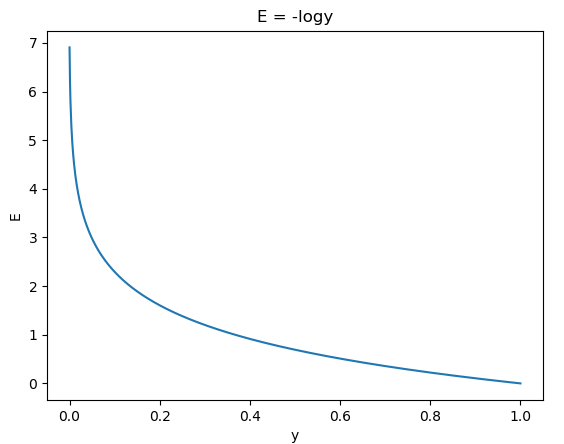
\includegraphics[width=7cm]{./figure./graph2_2.png}
\end{center}
\caption{交差エントロピー誤差2}
\end{figure}

$交差エントロピー誤差はソフトマックス関数と組み合わせて使うことが多いため、y,tはそれぞれ(0\le y \le 1)\ , (0\le t \le 1)となり、確率のように扱える。交差エントロピー誤差はyがtに近い値を出力するほど値が小さくなっていく。交差エントロピー誤差の最小値はy=1、つまりy=tになる時に最小値をとる。またy=0の時は損失関数の値が∞に発散してしまうので、実装する際にはyに微小な値を足し合わせることで発散を防ぐ。$
\begin{flushright}
\bunseki{※伊藤晋之介}
\end{flushright}

\subsection{パラメータの更新}

ニューラルネットワークのパラメータには次のようなものがある。

\begin{itemize}
\item 重みパラメータ \sl{W}
\item バイアス \sl{b}
\end{itemize}

これらのパラメータを損失関数をもとに更新していく。具体的には損失関数が最小になるようなパラメータを設定していく。しかし一般的には損失関数は複雑であり、ニューラルネットワークのパラメータも層が増えるにつれて数が膨大になっていく。そのため損失関数が最小になる点を求めるのは簡単ではない。そこで損失関数が最小となる点を求めるために用いられる方法の一つに勾配降下法がある。

\begin{flushright}
\bunseki{※伊藤晋之介}
\end{flushright}

\subsubsection{勾配降下法}
勾配降下法とは関数の最小値を求めるためのアルゴリズムであり、以下の式で表される。
\begin{itemize}
\item{$ある関数がy=f(x)となる時$}
\end{itemize}
\begin{equation}
x_{t+1}=x_t - \eta\frac{\partial f(x_t)}{\partial x}
\end{equation}

$ここで\frac{\partial f(x_t)}{\partial x}はある点x_tでのf(x)の勾配を表す。$
$また\mu は学習率といい、一度の更新でどれだけパラメータを更新するかを決めるものである。この値は大きすぎても小さすぎても学習がうまくいかなくなってしまう。そのため様々な値を試し、適当な大きさに設定していく必要がある。$
具体的な手順は次のようになる。

\begin{enumerate}
\item{ある点xでの関数の勾配を偏微分で求める}
\item{その点から勾配を減らす方向に進む}
\item{上の2つを一定の回数繰り返していく}
\end{enumerate}

$ここでは実際にz=f(x,y)、f(x,y)=x^2+y^2の最小値を勾配法で求めてみる。
x,yの更新式は次のようになる。$
\begin{equation}
x_{t+1} =x_t - \eta \frac{\partial f(x_t,y_t)}{\partial x},\ 
y_{t+1} =y_t - \eta \frac{\partial f(x_t,y_t)}{\partial y}
\end{equation}
$xの初期値x_0=1.7、yの初期値y_0=1.7、学習率\eta = 0.1として勾配法のアルゴリズムを適用すると次のようになる。$

\begin{figure}[h]
\begin{center}
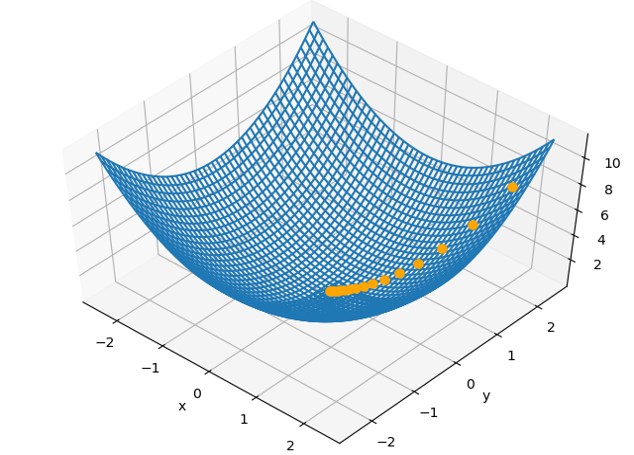
\includegraphics[width=7cm]{./figure./graph3.png}
\end{center}
\caption{勾配降下法の例}
\end{figure}

$f(x,y) = x^2 + y^2の最小値は(x,y)=(0,0)、勾配降下法を用いることで確かに最小値を求めることができることがわかる。$

$ニューラルネットワークの場合の勾配ついて説明していく。ニューラルネットワークの勾配とは重みパラメータに関する損失関数の勾配である。例えば2×3の重みWをもつニューラルネットワークの場合を考える。この時損失関数に対する各重みの勾配\frac{\partial E}{\partial W}は図のようになる。$

\[
  W = \left(
    \begin{array}{ccc}
      W_{11} & W_{12} & W_{13} \\
      W_{21} & W_{22} & W_{23} 
    \end{array}
  \right)
\]

\[
  \frac{\partial E}{\partial W} = \left(
    \begin{array}{ccc}
     \frac{\partial E}{\partial W_{11}} & \frac{\partial E}{\partial W_{12}} & \frac{\partial E}{\partial W_{13}} \\
\\
      \frac{\partial E}{\partial W_{21}} & \frac{\partial E}{\partial W_{22}} & \frac{\partial E}{\partial W_{23}} 
    \end{array}
  \right)
\]
$\frac{\partial E}{\partial W}の各要素はそれぞれの要素の偏微分から構成される。例えば1行目1列目の\frac{\partial E}{\partial W_{11}}はW_{11}の値を変えた場合の数値微分を求めパラメータを更新する。これを各パラメータに対して行う。$

\begin{flushright}
\bunseki{※伊藤晋之介}
\end{flushright}

\subsection{誤差逆伝播法}
$数値微分でのパラメータの更新は簡単だが計算に時間がかかる。そこでより効率的に計算を行うことができる誤差逆伝播法について説明する。
誤差逆伝播法はニューラルネットワークの出力から損失関数の微分値を入力側へ伝えていく。そうすることで一度の実行で損失関数の各層に対する微分を求めることができるようになる。数値微分と誤差逆伝播法の計算量の違いを比較する。$

数値微分\\
\begin{itemize}
\item{数値微分の場合の計算量はニューラルネットワークのパラメータ量に比例する。}
\item{Nをニューラルネットワークのパラメータ量とする}
\item{$一回の実行にかかる計算量はCN(C:定数)$}
\item{更新するパラメータの数だけ実行する必要がある。}
\item{$最終的な計算量はO(N^2)となる。$}
\end{itemize}

誤差逆伝播法
\begin{itemize}
\item{一度の学習で全てのパラメータを更新することができる。}
\item{パラメータの更新回数はパラメータの量に比例する}
\item{$一度の実行にかかる計算量をCN(C:定数)とする$}
\item{$最終的な計算量はO(N)となる。$}

このため誤差逆伝播法を使うことで効率よくパラメータを更新することができる。
\end{itemize}
\begin{flushright}
\bunseki{※伊藤晋之介}
\end{flushright}